%!TEX root = paper.tex

Rather than looking at the explicit representation equation of lines in the plane, we can gain much more insight from looking at the parametric representation. To simplify our analysis, we will choose our time parameter such that v collisions occur every $\Delta t = 1$ and h collisions occur every $\Delta t = m$. The equation for a line $y(x) = m \, x + y_0$ is equivalent to the following parametric system

\begin{align}\label{eq:parametric-line}
	x_0& \coloneqq - \frac{y_0}{m}\\
	x(t)& = \frac{1}{m} \, t + x_0\\
	y(t)& = t
\end{align}

Now v and h collisions in the 2-dimensional plane can be projected onto the 1-dimensional $t$ axis. The problem of mapping collision sequences to lines in the plane becomes a problem of fitting tick marks with regular spacing $1$ into intervals of length $m$.

\begin{figure}[H]
  \begin{center}
    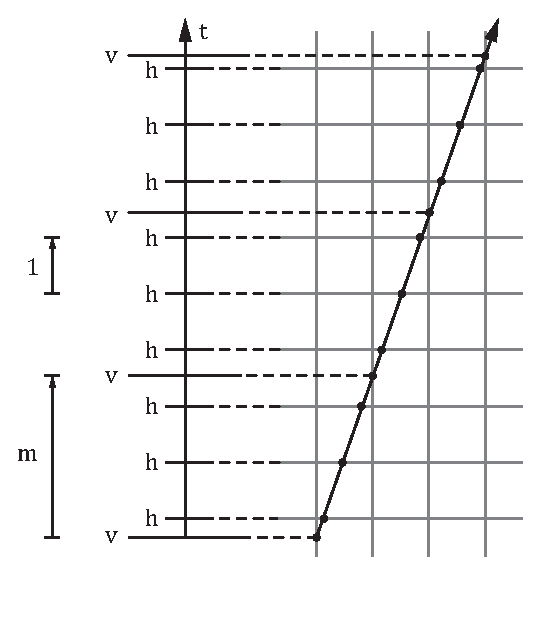
\includegraphics[keepaspectratio, height=4in]{1d_mapping_1}
  \end{center}
  \vspace{-.2in} % corrects bad spacing
  \caption{\label{fig:1d-projection} Projecting onto the parametric representation.}
\end{figure}

For the sake of space, we will rotate the $t$ axis so that it is horizontal.

\begin{figure}[H]
  \begin{center}
    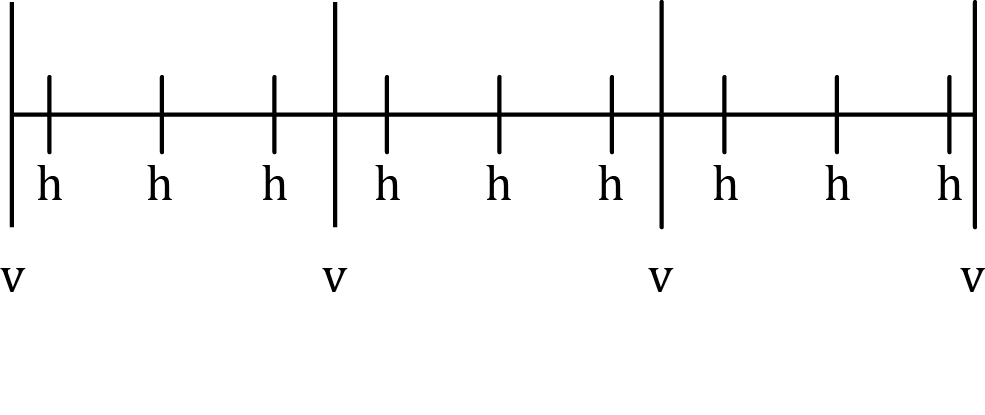
\includegraphics[keepaspectratio, width=4in]{1d_mapping_2}
  \end{center}
  \vspace{-.2in} % corrects bad spacing
  \caption{\label{fig:1d-problem} An example collision sequence.}
\end{figure}

% -----------------------------------------------------------------------------

\begin{lemma}\label{lem:interval-ticks}
	Let $l_2 < l_1$. The number of real numbers at regular spacing $l_2$ inside an open interval of length $l_1$ is in $\cbracket{\floor{\frac{l_1}{l_2}}, \ceil{\frac{l_1}{l_2}}}$.
\end{lemma}

\begin{proof}
	Let $A \subset \Z$ represent the set of all possible numbers of real numbers at regular spacing $l_2$ inside an open interval of length $l_1$. Given some $a \in A$, let $b \in \R$ be defined such that the following holds

	\begin{equation}\label{eq:interval-ticks}
		l_1 = (a - 1) l_2 + b
	\end{equation}

	We know that $(a - 1) l_2 < l_1$, so $b \ge 0$. Also, $b < 2 \, l_2$ because otherwise, there must be more than $a$ real numbers inside the interval, contradicting our original assumption.

	Rearranging Equation \ref{eq:interval-ticks}, we get

	\begin{gather}
		a = \frac{l_1}{l_2} + 1 - \frac{b}{l_2}\\
		\frac{l_1}{l_2} - 1 < a < \frac{l_1}{l_2} + 1\\
		a \in \cbracket{\floor{\frac{l_1}{l_2}}, \ceil{\frac{l_1}{l_2}}}
	\end{gather}
\end{proof}
